% Options for packages loaded elsewhere
\PassOptionsToPackage{unicode}{hyperref}
\PassOptionsToPackage{hyphens}{url}
%
\documentclass[
]{article}
\usepackage{amsmath,amssymb}
\usepackage{iftex}
\ifPDFTeX
  \usepackage[T1]{fontenc}
  \usepackage[utf8]{inputenc}
  \usepackage{textcomp} % provide euro and other symbols
\else % if luatex or xetex
  \usepackage{unicode-math} % this also loads fontspec
  \defaultfontfeatures{Scale=MatchLowercase}
  \defaultfontfeatures[\rmfamily]{Ligatures=TeX,Scale=1}
\fi
\usepackage{lmodern}
\ifPDFTeX\else
  % xetex/luatex font selection
\fi
% Use upquote if available, for straight quotes in verbatim environments
\IfFileExists{upquote.sty}{\usepackage{upquote}}{}
\IfFileExists{microtype.sty}{% use microtype if available
  \usepackage[]{microtype}
  \UseMicrotypeSet[protrusion]{basicmath} % disable protrusion for tt fonts
}{}
\makeatletter
\@ifundefined{KOMAClassName}{% if non-KOMA class
  \IfFileExists{parskip.sty}{%
    \usepackage{parskip}
  }{% else
    \setlength{\parindent}{0pt}
    \setlength{\parskip}{6pt plus 2pt minus 1pt}}
}{% if KOMA class
  \KOMAoptions{parskip=half}}
\makeatother
\usepackage{xcolor}
\usepackage[margin=1in]{geometry}
\usepackage{color}
\usepackage{fancyvrb}
\newcommand{\VerbBar}{|}
\newcommand{\VERB}{\Verb[commandchars=\\\{\}]}
\DefineVerbatimEnvironment{Highlighting}{Verbatim}{commandchars=\\\{\}}
% Add ',fontsize=\small' for more characters per line
\usepackage{framed}
\definecolor{shadecolor}{RGB}{248,248,248}
\newenvironment{Shaded}{\begin{snugshade}}{\end{snugshade}}
\newcommand{\AlertTok}[1]{\textcolor[rgb]{0.94,0.16,0.16}{#1}}
\newcommand{\AnnotationTok}[1]{\textcolor[rgb]{0.56,0.35,0.01}{\textbf{\textit{#1}}}}
\newcommand{\AttributeTok}[1]{\textcolor[rgb]{0.13,0.29,0.53}{#1}}
\newcommand{\BaseNTok}[1]{\textcolor[rgb]{0.00,0.00,0.81}{#1}}
\newcommand{\BuiltInTok}[1]{#1}
\newcommand{\CharTok}[1]{\textcolor[rgb]{0.31,0.60,0.02}{#1}}
\newcommand{\CommentTok}[1]{\textcolor[rgb]{0.56,0.35,0.01}{\textit{#1}}}
\newcommand{\CommentVarTok}[1]{\textcolor[rgb]{0.56,0.35,0.01}{\textbf{\textit{#1}}}}
\newcommand{\ConstantTok}[1]{\textcolor[rgb]{0.56,0.35,0.01}{#1}}
\newcommand{\ControlFlowTok}[1]{\textcolor[rgb]{0.13,0.29,0.53}{\textbf{#1}}}
\newcommand{\DataTypeTok}[1]{\textcolor[rgb]{0.13,0.29,0.53}{#1}}
\newcommand{\DecValTok}[1]{\textcolor[rgb]{0.00,0.00,0.81}{#1}}
\newcommand{\DocumentationTok}[1]{\textcolor[rgb]{0.56,0.35,0.01}{\textbf{\textit{#1}}}}
\newcommand{\ErrorTok}[1]{\textcolor[rgb]{0.64,0.00,0.00}{\textbf{#1}}}
\newcommand{\ExtensionTok}[1]{#1}
\newcommand{\FloatTok}[1]{\textcolor[rgb]{0.00,0.00,0.81}{#1}}
\newcommand{\FunctionTok}[1]{\textcolor[rgb]{0.13,0.29,0.53}{\textbf{#1}}}
\newcommand{\ImportTok}[1]{#1}
\newcommand{\InformationTok}[1]{\textcolor[rgb]{0.56,0.35,0.01}{\textbf{\textit{#1}}}}
\newcommand{\KeywordTok}[1]{\textcolor[rgb]{0.13,0.29,0.53}{\textbf{#1}}}
\newcommand{\NormalTok}[1]{#1}
\newcommand{\OperatorTok}[1]{\textcolor[rgb]{0.81,0.36,0.00}{\textbf{#1}}}
\newcommand{\OtherTok}[1]{\textcolor[rgb]{0.56,0.35,0.01}{#1}}
\newcommand{\PreprocessorTok}[1]{\textcolor[rgb]{0.56,0.35,0.01}{\textit{#1}}}
\newcommand{\RegionMarkerTok}[1]{#1}
\newcommand{\SpecialCharTok}[1]{\textcolor[rgb]{0.81,0.36,0.00}{\textbf{#1}}}
\newcommand{\SpecialStringTok}[1]{\textcolor[rgb]{0.31,0.60,0.02}{#1}}
\newcommand{\StringTok}[1]{\textcolor[rgb]{0.31,0.60,0.02}{#1}}
\newcommand{\VariableTok}[1]{\textcolor[rgb]{0.00,0.00,0.00}{#1}}
\newcommand{\VerbatimStringTok}[1]{\textcolor[rgb]{0.31,0.60,0.02}{#1}}
\newcommand{\WarningTok}[1]{\textcolor[rgb]{0.56,0.35,0.01}{\textbf{\textit{#1}}}}
\usepackage{graphicx}
\makeatletter
\def\maxwidth{\ifdim\Gin@nat@width>\linewidth\linewidth\else\Gin@nat@width\fi}
\def\maxheight{\ifdim\Gin@nat@height>\textheight\textheight\else\Gin@nat@height\fi}
\makeatother
% Scale images if necessary, so that they will not overflow the page
% margins by default, and it is still possible to overwrite the defaults
% using explicit options in \includegraphics[width, height, ...]{}
\setkeys{Gin}{width=\maxwidth,height=\maxheight,keepaspectratio}
% Set default figure placement to htbp
\makeatletter
\def\fps@figure{htbp}
\makeatother
\setlength{\emergencystretch}{3em} % prevent overfull lines
\providecommand{\tightlist}{%
  \setlength{\itemsep}{0pt}\setlength{\parskip}{0pt}}
\setcounter{secnumdepth}{-\maxdimen} % remove section numbering
\usepackage{booktabs}
\usepackage{longtable}
\usepackage{array}
\usepackage{multirow}
\usepackage{wrapfig}
\usepackage{float}
\usepackage{colortbl}
\usepackage{pdflscape}
\usepackage{tabu}
\usepackage{threeparttable}
\usepackage{threeparttablex}
\usepackage[normalem]{ulem}
\usepackage{makecell}
\usepackage{xcolor}
\ifLuaTeX
  \usepackage{selnolig}  % disable illegal ligatures
\fi
\IfFileExists{bookmark.sty}{\usepackage{bookmark}}{\usepackage{hyperref}}
\IfFileExists{xurl.sty}{\usepackage{xurl}}{} % add URL line breaks if available
\urlstyle{same}
\hypersetup{
  pdftitle={DATA 621 HW 3 Crime},
  pdfauthor={Jian Quan Chen, Frederick Jones},
  hidelinks,
  pdfcreator={LaTeX via pandoc}}

\title{DATA 621 HW 3 Crime}
\author{Jian Quan Chen, Frederick Jones}
\date{2024-03-22}

\begin{document}
\maketitle

\hypertarget{data-exploration}{%
\section{1. Data Exploration}\label{data-exploration}}

\begin{Shaded}
\begin{Highlighting}[]
\FunctionTok{library}\NormalTok{(tidyverse)}
\FunctionTok{library}\NormalTok{(psych)}
\FunctionTok{library}\NormalTok{(corrplot)}
\FunctionTok{library}\NormalTok{(MASS)}
\FunctionTok{library}\NormalTok{(pROC)}
\FunctionTok{library}\NormalTok{(kableExtra)}
\FunctionTok{library}\NormalTok{(caret)}
\end{Highlighting}
\end{Shaded}

\begin{Shaded}
\begin{Highlighting}[]
\NormalTok{df }\OtherTok{\textless{}{-}} \FunctionTok{read.csv}\NormalTok{(}\StringTok{"https://raw.githubusercontent.com/LeJQC/DATA{-}621{-}Group{-}2/main/HW3/crime{-}training{-}data\_modified.csv"}\NormalTok{)}
\end{Highlighting}
\end{Shaded}

Let's get a general sense of the training data set using the
\texttt{glimpse} function. There are 466 observations and 13 variables
in the training data set. Of the 13 variables, 12 are predictor
variables and 1 is the target variable. All of the variables seem to be
floats or integers.

\begin{Shaded}
\begin{Highlighting}[]
\FunctionTok{glimpse}\NormalTok{(df)}
\end{Highlighting}
\end{Shaded}

\begin{verbatim}
## Rows: 466
## Columns: 13
## $ zn      <dbl> 0, 0, 0, 30, 0, 0, 0, 0, 0, 80, 22, 0, 0, 22, 0, 0, 100, 20, 0~
## $ indus   <dbl> 19.58, 19.58, 18.10, 4.93, 2.46, 8.56, 18.10, 18.10, 5.19, 3.6~
## $ chas    <int> 0, 1, 0, 0, 0, 0, 0, 0, 0, 0, 0, 0, 0, 0, 0, 0, 0, 0, 0, 0, 0,~
## $ nox     <dbl> 0.605, 0.871, 0.740, 0.428, 0.488, 0.520, 0.693, 0.693, 0.515,~
## $ rm      <dbl> 7.929, 5.403, 6.485, 6.393, 7.155, 6.781, 5.453, 4.519, 6.316,~
## $ age     <dbl> 96.2, 100.0, 100.0, 7.8, 92.2, 71.3, 100.0, 100.0, 38.1, 19.1,~
## $ dis     <dbl> 2.0459, 1.3216, 1.9784, 7.0355, 2.7006, 2.8561, 1.4896, 1.6582~
## $ rad     <int> 5, 5, 24, 6, 3, 5, 24, 24, 5, 1, 7, 5, 24, 7, 3, 3, 5, 5, 24, ~
## $ tax     <int> 403, 403, 666, 300, 193, 384, 666, 666, 224, 315, 330, 398, 66~
## $ ptratio <dbl> 14.7, 14.7, 20.2, 16.6, 17.8, 20.9, 20.2, 20.2, 20.2, 16.4, 19~
## $ lstat   <dbl> 3.70, 26.82, 18.85, 5.19, 4.82, 7.67, 30.59, 36.98, 5.68, 9.25~
## $ medv    <dbl> 50.0, 13.4, 15.4, 23.7, 37.9, 26.5, 5.0, 7.0, 22.2, 20.9, 24.8~
## $ target  <int> 1, 1, 1, 0, 0, 0, 1, 1, 0, 0, 0, 0, 1, 1, 0, 0, 0, 1, 1, 1, 0,~
\end{verbatim}

The variables are:

\begin{itemize}
\tightlist
\item
  \texttt{zn}: proportion of residential land zoned for large lots (over
  25000 square feet)
\item
  \texttt{indus}: proportion of non-retail business acres per suburb
\item
  \texttt{chas}: a dummy var. for whether the suburb borders the Charles
  River (1) or not (0)
\item
  \texttt{nox}: nitrogen oxides concentration (parts per 10 million)
\item
  \texttt{rm}: average number of rooms per dwelling
\item
  \texttt{age}: proportion of owner-occupied units built prior to 1940
\item
  \texttt{dis}: weighted mean of distances to five Boston employment
  centers
\item
  \texttt{rad}: index of accessibility to radial highways
\item
  \texttt{tax}: full-value property-tax rate per \$10,000
\item
  \texttt{ptratio}: pupil-teacher ratio by town
\item
  \texttt{lstat}: lower status of the population (percent)
\item
  \texttt{medv}: median value of owner-occupied homes in \$1000s
\item
  \texttt{target}: whether the crime rate is above the median crime rate
  (1) or not (0)
\end{itemize}

\hypertarget{summary-table}{%
\subsection{Summary Table}\label{summary-table}}

Using the \texttt{describe} function from the psych library, we can get
the summary statistics of all the variables as shown in the table below.
Something to note here is the large standard deviation with the
\texttt{zn}, \texttt{age} variable compared to its range, which may be
because they are proportions. Another thing that stands out is the
\texttt{tax} variable. The mean, standard deviation, median, and range
are much larger than the other predictor variables so we might have to
do some transformation on it later on.

\begin{Shaded}
\begin{Highlighting}[]
\NormalTok{summary\_table }\OtherTok{\textless{}{-}} \FunctionTok{describe}\NormalTok{(df)}

\FunctionTok{print}\NormalTok{(}\FunctionTok{round}\NormalTok{(summary\_table,}\DecValTok{2}\NormalTok{))}
\end{Highlighting}
\end{Shaded}

\begin{verbatim}
##         vars   n   mean     sd median trimmed    mad    min    max  range  skew
## zn         1 466  11.58  23.36   0.00    5.35   0.00   0.00 100.00 100.00  2.18
## indus      2 466  11.11   6.85   9.69   10.91   9.34   0.46  27.74  27.28  0.29
## chas       3 466   0.07   0.26   0.00    0.00   0.00   0.00   1.00   1.00  3.34
## nox        4 466   0.55   0.12   0.54    0.54   0.13   0.39   0.87   0.48  0.75
## rm         5 466   6.29   0.70   6.21    6.26   0.52   3.86   8.78   4.92  0.48
## age        6 466  68.37  28.32  77.15   70.96  30.02   2.90 100.00  97.10 -0.58
## dis        7 466   3.80   2.11   3.19    3.54   1.91   1.13  12.13  11.00  1.00
## rad        8 466   9.53   8.69   5.00    8.70   1.48   1.00  24.00  23.00  1.01
## tax        9 466 409.50 167.90 334.50  401.51 104.52 187.00 711.00 524.00  0.66
## ptratio   10 466  18.40   2.20  18.90   18.60   1.93  12.60  22.00   9.40 -0.75
## lstat     11 466  12.63   7.10  11.35   11.88   7.07   1.73  37.97  36.24  0.91
## medv      12 466  22.59   9.24  21.20   21.63   6.00   5.00  50.00  45.00  1.08
## target    13 466   0.49   0.50   0.00    0.49   0.00   0.00   1.00   1.00  0.03
##         kurtosis   se
## zn          3.81 1.08
## indus      -1.24 0.32
## chas        9.15 0.01
## nox        -0.04 0.01
## rm          1.54 0.03
## age        -1.01 1.31
## dis         0.47 0.10
## rad        -0.86 0.40
## tax        -1.15 7.78
## ptratio    -0.40 0.10
## lstat       0.50 0.33
## medv        1.37 0.43
## target     -2.00 0.02
\end{verbatim}

\hypertarget{distrubtion-plot}{%
\subsection{Distrubtion Plot}\label{distrubtion-plot}}

Next, let's look at the distribution of the 13 variables. As expected
the values of the target variable are distributed around 0 and 1.
Variables such as age, chas, dis, lstat, nox, ptration, rad, and zn are
skewed to the left or right. On the other hand, variables medv and rm
are normally distributed. The remaining predictor variables indus and
tax have a bimodal distribution curve.

\begin{Shaded}
\begin{Highlighting}[]
\NormalTok{df\_long }\OtherTok{\textless{}{-}}\NormalTok{ df }\SpecialCharTok{\%\textgreater{}\%}
  \FunctionTok{pivot\_longer}\NormalTok{(}
    \AttributeTok{cols =} \FunctionTok{everything}\NormalTok{(), }
    \AttributeTok{names\_to =} \StringTok{"variable"}\NormalTok{,}
    \AttributeTok{values\_to =} \StringTok{"value"}
\NormalTok{  )}

\NormalTok{df\_long }\SpecialCharTok{\%\textgreater{}\%}
  \FunctionTok{ggplot}\NormalTok{(}\FunctionTok{aes}\NormalTok{(value)) }\SpecialCharTok{+} 
  \FunctionTok{geom\_density}\NormalTok{(}\AttributeTok{fill =} \StringTok{"blue"}\NormalTok{) }\SpecialCharTok{+} 
  \FunctionTok{facet\_wrap}\NormalTok{(}\SpecialCharTok{\textasciitilde{}}\NormalTok{variable, }\AttributeTok{scales =}\StringTok{"free"}\NormalTok{, }\AttributeTok{ncol =} \DecValTok{4}\NormalTok{) }\SpecialCharTok{+}
  \FunctionTok{labs}\NormalTok{(}\AttributeTok{x =} \FunctionTok{element\_blank}\NormalTok{(), }\AttributeTok{y =} \FunctionTok{element\_blank}\NormalTok{())}
\end{Highlighting}
\end{Shaded}

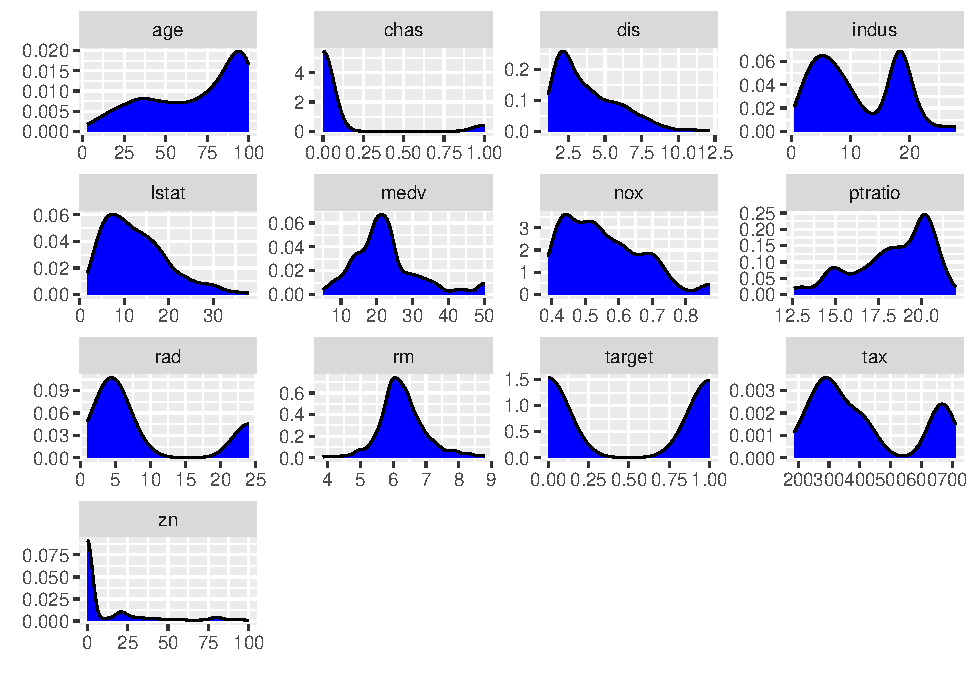
\includegraphics{HW-3-Crime-FINAL_files/figure-latex/unnamed-chunk-5-1.pdf}

\hypertarget{correlation-plot}{%
\subsection{Correlation Plot}\label{correlation-plot}}

To identify the correlation between each variable we can create a
correlation plot by using the corrplot library. According to the
correlation plot, the variables nox (0.73), age (0.63), rad (0.63), tax
(0.61), and indus (0.60) are most linearly correlated with the target
variable. In addition, there is a high degree of collinearity with tax
and rad (0.91) and with nox and indus (0.76). These are variables to
keep in mind when we select variables for our models.

\begin{Shaded}
\begin{Highlighting}[]
\NormalTok{df }\SpecialCharTok{\%\textgreater{}\%} 
  \FunctionTok{cor}\NormalTok{(}\AttributeTok{use =} \StringTok{"complete.obs"}\NormalTok{) }\SpecialCharTok{\%\textgreater{}\%}
  \FunctionTok{corrplot}\NormalTok{(}\AttributeTok{method =} \StringTok{"color"}\NormalTok{, }\AttributeTok{tl.col =} \StringTok{"black"}\NormalTok{, }\AttributeTok{addCoef.col =} \StringTok{"black"}\NormalTok{, }\AttributeTok{number.cex =} \FloatTok{0.5}\NormalTok{)}
\end{Highlighting}
\end{Shaded}

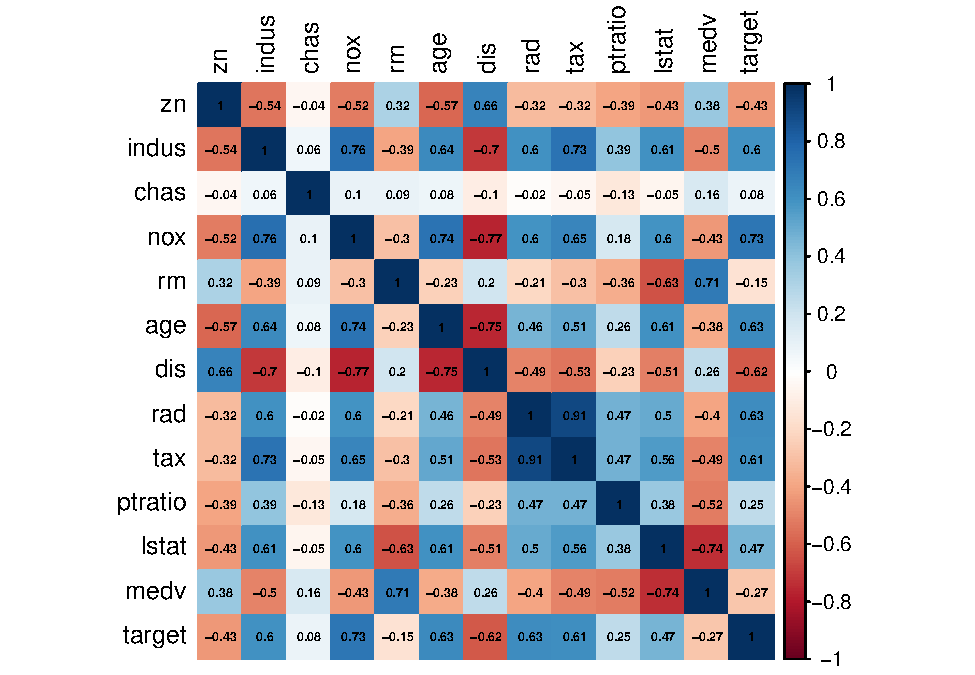
\includegraphics{HW-3-Crime-FINAL_files/figure-latex/unnamed-chunk-6-1.pdf}

\hypertarget{boxplot}{%
\subsection{Boxplot}\label{boxplot}}

This boxplot shows the distribution and quartile ranges of the
variables. We see that there are obvious outliers in chas and dis, which
we may have to deal with later on. Other predictor variables such as
lstat, medv, rm, and zn also have outliers, which may need to be dealth
with later as well.

\begin{Shaded}
\begin{Highlighting}[]
\NormalTok{df\_long }\SpecialCharTok{\%\textgreater{}\%} 
  \FunctionTok{ggplot}\NormalTok{(}\FunctionTok{aes}\NormalTok{(variable, value)) }\SpecialCharTok{+} 
  \FunctionTok{geom\_boxplot}\NormalTok{() }\SpecialCharTok{+} 
  \FunctionTok{facet\_wrap}\NormalTok{(}\SpecialCharTok{\textasciitilde{}}\NormalTok{variable, }\AttributeTok{scales=}\StringTok{\textquotesingle{}free\textquotesingle{}}\NormalTok{, }\AttributeTok{ncol=}\DecValTok{5}\NormalTok{)}
\end{Highlighting}
\end{Shaded}

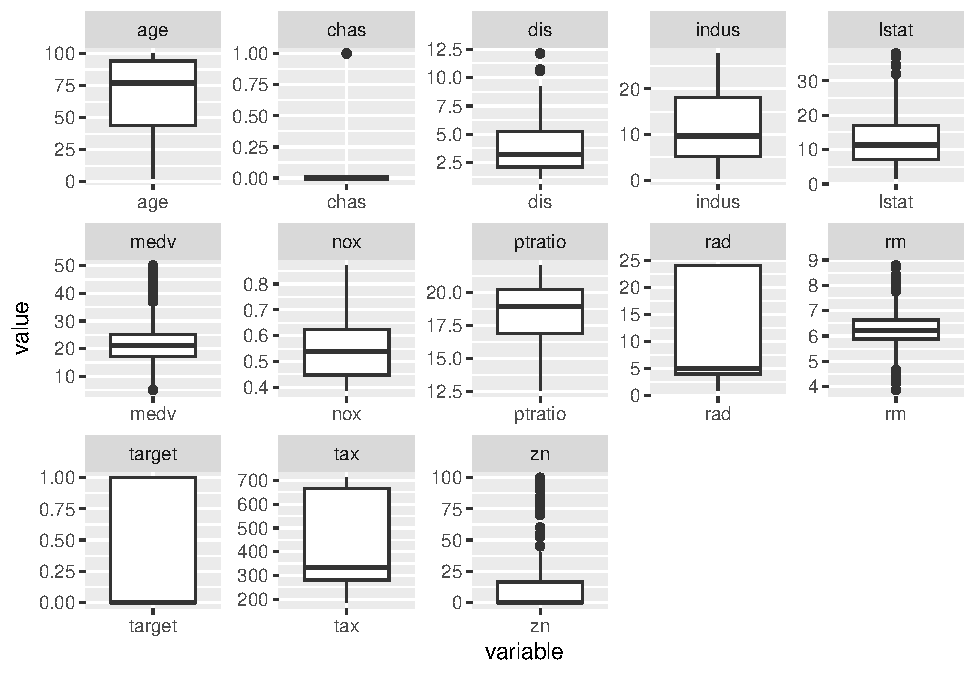
\includegraphics{HW-3-Crime-FINAL_files/figure-latex/unnamed-chunk-7-1.pdf}

\hypertarget{data-preparation}{%
\section{2. Data Preparation}\label{data-preparation}}

\hypertarget{fix-any-missing-value-in-the-data}{%
\subsection{Fix any missing value in the
data}\label{fix-any-missing-value-in-the-data}}

\textbf{Let's check if there exists a null value or NA in the dataframe.
If Null is found it can be fixed using mean or median of the column in
which na is found.} \textbf{Attach the data}

\begin{Shaded}
\begin{Highlighting}[]
\NormalTok{training\_set }\OtherTok{\textless{}{-}}\NormalTok{ df}
\CommentTok{\#test\_set \textless{}{-} read.csv("https://raw.githubusercontent.com/LeJQC/DATA{-}621{-}Group{-}2/14f8d86b73472ac8f9302415a7e4c24b37052ea6/HW3/crime{-}evaluation{-}data\_modified.csv")}
\NormalTok{test\_set }\OtherTok{\textless{}{-}} \FunctionTok{read.csv}\NormalTok{(}\StringTok{"crime{-}evaluation{-}data\_modified.csv"}\NormalTok{)}
\end{Highlighting}
\end{Shaded}

\begin{Shaded}
\begin{Highlighting}[]
\FunctionTok{print}\NormalTok{(}\FunctionTok{sum}\NormalTok{(}\FunctionTok{is.na}\NormalTok{(training\_set)))}
\end{Highlighting}
\end{Shaded}

\begin{verbatim}
## [1] 0
\end{verbatim}

\begin{Shaded}
\begin{Highlighting}[]
\FunctionTok{print}\NormalTok{(}\FunctionTok{sum}\NormalTok{(}\FunctionTok{is.na}\NormalTok{(test\_set)))}
\end{Highlighting}
\end{Shaded}

\begin{verbatim}
## [1] 0
\end{verbatim}

This shows that there no missing value in the data and thus no need to
bother about the missing values.

\hypertarget{modify-an-existing-variable-or-create-a-new-variable-by-combining-the-two-or-more-variables}{%
\subsection{Modify an existing variable or create a new variable by
combining the two or more
variables}\label{modify-an-existing-variable-or-create-a-new-variable-by-combining-the-two-or-more-variables}}

It is to be noted that the tax column contain the tax rate per \$10,000
and medv contain the property value in \$1000. The median tax on
properties in neighborhood can be calculated by usingthese two columns.
\[medTax = \frac{medv*1000}{10000}*Tax\] or in simple it can be written
as medTax = medv\emph{Tax}1000/10000 = medv*tax/10

\begin{Shaded}
\begin{Highlighting}[]
\NormalTok{training\_set}\OtherTok{\textless{}{-}}\NormalTok{ training\_set}\SpecialCharTok{|\textgreater{}}\FunctionTok{mutate}\NormalTok{(}
  \AttributeTok{medTax =}\NormalTok{ medv}\SpecialCharTok{*}\NormalTok{tax}\SpecialCharTok{/}\DecValTok{10}
\NormalTok{)}\SpecialCharTok{|\textgreater{}}
  \FunctionTok{relocate}\NormalTok{(medTax, }\AttributeTok{.before =} \DecValTok{10}\NormalTok{)}
\NormalTok{test\_set}\OtherTok{\textless{}{-}}\NormalTok{ training\_set}\SpecialCharTok{|\textgreater{}}\FunctionTok{mutate}\NormalTok{(}
  \AttributeTok{medTax =}\NormalTok{ medv}\SpecialCharTok{*}\NormalTok{tax}\SpecialCharTok{/}\DecValTok{10}
\NormalTok{)}\SpecialCharTok{|\textgreater{}}\FunctionTok{relocate}\NormalTok{(medTax, }\AttributeTok{.before =} \DecValTok{10}\NormalTok{)}
\FunctionTok{head}\NormalTok{(training\_set)}
\end{Highlighting}
\end{Shaded}

\begin{verbatim}
##   zn indus chas   nox    rm   age    dis rad tax  medTax ptratio lstat medv
## 1  0 19.58    0 0.605 7.929  96.2 2.0459   5 403 2015.00    14.7  3.70 50.0
## 2  0 19.58    1 0.871 5.403 100.0 1.3216   5 403  540.02    14.7 26.82 13.4
## 3  0 18.10    0 0.740 6.485 100.0 1.9784  24 666 1025.64    20.2 18.85 15.4
## 4 30  4.93    0 0.428 6.393   7.8 7.0355   6 300  711.00    16.6  5.19 23.7
## 5  0  2.46    0 0.488 7.155  92.2 2.7006   3 193  731.47    17.8  4.82 37.9
## 6  0  8.56    0 0.520 6.781  71.3 2.8561   5 384 1017.60    20.9  7.67 26.5
##   target
## 1      1
## 2      1
## 3      1
## 4      0
## 5      0
## 6      0
\end{verbatim}

\hypertarget{feature-scaling}{%
\subsection{Feature scaling}\label{feature-scaling}}

\textbf{Now the data can be scaled so that the all the predictors have
equal effect on the response variable.}

It can concluded from the summary table that the range of some variable
is high like zn's range is 0-100. This range can be normalize or
standardize so that the range is between 0 and 1 or -3 to 3
respectively.

To normalize a number we just divide it by the maximum value in the
variable. This can be done conviniently using scale() function in R.

Note: No need to standardize the target variable, the predictor
variables chas and nox because these already contain 0 and 1 or within
the standardized limit.

\begin{Shaded}
\begin{Highlighting}[]
\NormalTok{training\_set[,}\DecValTok{1}\SpecialCharTok{:}\DecValTok{12}\NormalTok{][,}\FunctionTok{c}\NormalTok{(}\SpecialCharTok{{-}}\DecValTok{3}\NormalTok{, }\SpecialCharTok{{-}}\DecValTok{4}\NormalTok{)] }\OtherTok{=} \FunctionTok{scale}\NormalTok{(training\_set[, }\DecValTok{1}\SpecialCharTok{:}\DecValTok{12}\NormalTok{][,}\FunctionTok{c}\NormalTok{(}\SpecialCharTok{{-}}\DecValTok{3}\NormalTok{, }\SpecialCharTok{{-}}\DecValTok{4}\NormalTok{)])}
\NormalTok{test\_set }\OtherTok{=} \FunctionTok{scale}\NormalTok{(test\_set)}
\FunctionTok{head}\NormalTok{(training\_set)}
\end{Highlighting}
\end{Shaded}

\begin{verbatim}
##           zn      indus chas   nox         rm        age        dis        rad
## 1 -0.4955029  1.2379723    0 0.605  2.3243572  0.9827348 -0.8304864 -0.5215382
## 2 -0.4955029  1.2379723    1 0.871 -1.2593775  1.1169090 -1.1742535 -0.5215382
## 3 -0.4955029  1.0217831    0 0.740  0.2756981  1.1169090 -0.8625232  1.6659082
## 4  0.7884880 -0.9020088    0 0.428  0.1451741 -2.1385822  1.5376766 -0.4064095
## 5 -0.4955029 -1.2628111    0 0.488  1.2262532  0.8414987 -0.5197528 -0.7517957
## 6 -0.4955029 -0.3717609    0 0.520  0.6956449  0.1035403 -0.4459494 -0.5215382
##           tax     medTax    ptratio      lstat medv target
## 1 -0.03872628  3.0265702 -1.6835500 -1.2576171 50.0      1
## 2 -0.03872628 -0.8025987 -1.6835500  1.9978540 13.4      1
## 3  1.52768147  0.4581106  0.8200407  0.8756176 15.4      1
## 4 -0.65218635 -0.3587206 -0.8186732 -1.0478138 23.7      0
## 5 -1.28947011 -0.3055788 -0.2724352 -1.0999126 37.9      0
## 6 -0.15188882  0.4372381  1.1386795 -0.6986110 26.5      0
\end{verbatim}

\hypertarget{build-models-logistic-regression-binary-models}{%
\section{3. Build Models (Logistic regression binary
models)}\label{build-models-logistic-regression-binary-models}}

\hypertarget{model-1}{%
\subsection{Model 1}\label{model-1}}

The first task before writing the any model is to select the predictor
variables.But the seldction of suitable predictor variable is a complex
task and if we omit any predictor varible which influence the target
variable, it induces a bias in the output of the model which is known as
omitted-variable bias. Thus, one need to be very careful while selction
of suitable predictor variable.

We can use the most correlated variables with the target variable. Using
the scatterplot, it can be seen that the target variable is highly
correlated with the following variables:

indus, nox, age, rad, lstat

And weakly correlated with medTax, ptratio

And almost neutral with chas and highly negatively correlated with zn,
dis, medv, rm.

The correlation plot can be regenerated on the modified or transformed
data to see the correlation among the transformed variables.

\begin{Shaded}
\begin{Highlighting}[]
\NormalTok{training\_set }\SpecialCharTok{\%\textgreater{}\%} 
  \FunctionTok{cor}\NormalTok{(}\AttributeTok{use =} \StringTok{"complete.obs"}\NormalTok{) }\SpecialCharTok{\%\textgreater{}\%}
  \FunctionTok{corrplot}\NormalTok{(}\AttributeTok{method =} \StringTok{"color"}\NormalTok{, }\AttributeTok{tl.col =} \StringTok{"black"}\NormalTok{)}
\end{Highlighting}
\end{Shaded}

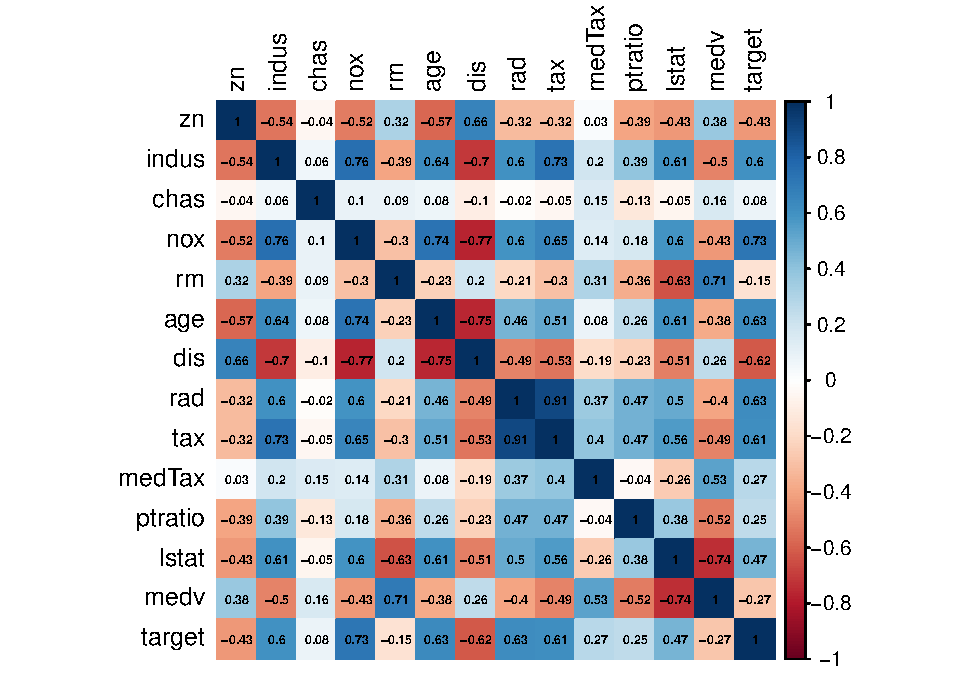
\includegraphics{HW-3-Crime-FINAL_files/figure-latex/unnamed-chunk-12-1.pdf}
The highly correlated components can be selected for the logistic
regression. Therefore, we will use indus, nox, age, rad, lstat, zn, dis.
It can be seen that zn is higly correlated with nox, indus, age,
dis,ptratio, lstate, medv. Therefore, it will be better to leave zn and
no need to include in in the regression.

\begin{Shaded}
\begin{Highlighting}[]
\NormalTok{logistic\_model }\OtherTok{\textless{}{-}}  \FunctionTok{glm}\NormalTok{(target }\SpecialCharTok{\textasciitilde{}}\NormalTok{ indus }\SpecialCharTok{+}\NormalTok{ nox }\SpecialCharTok{+}\NormalTok{ age }\SpecialCharTok{+}\NormalTok{ rad }\SpecialCharTok{+}\NormalTok{ lstat }\SpecialCharTok{+}\NormalTok{ dis,}\AttributeTok{data =}\NormalTok{ training\_set, }\AttributeTok{family =}\NormalTok{ binomial)}
\FunctionTok{summary}\NormalTok{(logistic\_model)}
\end{Highlighting}
\end{Shaded}

\begin{verbatim}
## 
## Call:
## glm(formula = target ~ indus + nox + age + rad + lstat + dis, 
##     family = binomial, data = training_set)
## 
## Coefficients:
##             Estimate Std. Error z value Pr(>|z|)    
## (Intercept) -18.5491     3.6085  -5.140 2.74e-07 ***
## indus        -0.7102     0.3000  -2.367   0.0179 *  
## nox          37.6649     6.8269   5.517 3.45e-08 ***
## age           0.6428     0.2906   2.212   0.0270 *  
## rad           4.0670     0.9554   4.257 2.07e-05 ***
## lstat        -0.1679     0.2489  -0.675   0.4999    
## dis           0.5745     0.3265   1.760   0.0785 .  
## ---
## Signif. codes:  0 '***' 0.001 '**' 0.01 '*' 0.05 '.' 0.1 ' ' 1
## 
## (Dispersion parameter for binomial family taken to be 1)
## 
##     Null deviance: 645.88  on 465  degrees of freedom
## Residual deviance: 226.60  on 459  degrees of freedom
## AIC: 240.6
## 
## Number of Fisher Scoring iterations: 8
\end{verbatim}

The p-value for the lstat is 0.4999 which is more than the critical
value 0.05 thus this variable must be omited from the regression.

\begin{Shaded}
\begin{Highlighting}[]
\NormalTok{logistic\_model }\OtherTok{\textless{}{-}}  \FunctionTok{glm}\NormalTok{(target }\SpecialCharTok{\textasciitilde{}}\NormalTok{ indus }\SpecialCharTok{+}\NormalTok{ nox }\SpecialCharTok{+}\NormalTok{ age }\SpecialCharTok{+}\NormalTok{ rad }\SpecialCharTok{+}\NormalTok{ dis,}\AttributeTok{data =}\NormalTok{ training\_set, }\AttributeTok{family =}\NormalTok{ binomial)}
\FunctionTok{summary}\NormalTok{(logistic\_model)}
\end{Highlighting}
\end{Shaded}

\begin{verbatim}
## 
## Call:
## glm(formula = target ~ indus + nox + age + rad + dis, family = binomial, 
##     data = training_set)
## 
## Coefficients:
##             Estimate Std. Error z value Pr(>|z|)    
## (Intercept) -18.3222     3.5812  -5.116 3.12e-07 ***
## indus        -0.7445     0.2953  -2.521   0.0117 *  
## nox          37.3437     6.7919   5.498 3.83e-08 ***
## age           0.5693     0.2693   2.114   0.0345 *  
## rad           4.1268     0.9609   4.295 1.75e-05 ***
## dis           0.5279     0.3210   1.645   0.1000    
## ---
## Signif. codes:  0 '***' 0.001 '**' 0.01 '*' 0.05 '.' 0.1 ' ' 1
## 
## (Dispersion parameter for binomial family taken to be 1)
## 
##     Null deviance: 645.88  on 465  degrees of freedom
## Residual deviance: 227.06  on 460  degrees of freedom
## AIC: 239.06
## 
## Number of Fisher Scoring iterations: 8
\end{verbatim}

All the probability of the coefficients are less than 0.05 thus, it can
be concluded that all the coefficients are significant for the
regression. \textbf{Test the hypothesis with chisq-test}

\begin{Shaded}
\begin{Highlighting}[]
\FunctionTok{anova}\NormalTok{(logistic\_model, }\AttributeTok{test=}\StringTok{"Chisq"}\NormalTok{)}
\end{Highlighting}
\end{Shaded}

\begin{verbatim}
## Analysis of Deviance Table
## 
## Model: binomial, link: logit
## 
## Response: target
## 
## Terms added sequentially (first to last)
## 
## 
##       Df Deviance Resid. Df Resid. Dev  Pr(>Chi)    
## NULL                    465     645.88              
## indus  1  192.641       464     453.23 < 2.2e-16 ***
## nox    1  165.125       463     288.11 < 2.2e-16 ***
## age    1    1.421       462     286.69    0.2333    
## rad    1   56.943       461     229.75 4.487e-14 ***
## dis    1    2.686       460     227.06    0.1012    
## ---
## Signif. codes:  0 '***' 0.001 '**' 0.01 '*' 0.05 '.' 0.1 ' ' 1
\end{verbatim}

The probability of dis is more than 0.05 thus the variable dis can be
removed from the model and we have the logistic model.

\begin{Shaded}
\begin{Highlighting}[]
\NormalTok{logistic\_model }\OtherTok{\textless{}{-}}  \FunctionTok{glm}\NormalTok{(target }\SpecialCharTok{\textasciitilde{}}\NormalTok{ indus }\SpecialCharTok{+}\NormalTok{ nox }\SpecialCharTok{+}\NormalTok{ age }\SpecialCharTok{+}\NormalTok{ rad, }\AttributeTok{data =}\NormalTok{ training\_set, }\AttributeTok{family =}\NormalTok{ binomial)}
\FunctionTok{anova}\NormalTok{(logistic\_model, }\AttributeTok{test=}\StringTok{"Chisq"}\NormalTok{)}
\end{Highlighting}
\end{Shaded}

\begin{verbatim}
## Analysis of Deviance Table
## 
## Model: binomial, link: logit
## 
## Response: target
## 
## Terms added sequentially (first to last)
## 
## 
##       Df Deviance Resid. Df Resid. Dev  Pr(>Chi)    
## NULL                    465     645.88              
## indus  1  192.641       464     453.23 < 2.2e-16 ***
## nox    1  165.125       463     288.11 < 2.2e-16 ***
## age    1    1.421       462     286.69    0.2333    
## rad    1   56.943       461     229.75 4.487e-14 ***
## ---
## Signif. codes:  0 '***' 0.001 '**' 0.01 '*' 0.05 '.' 0.1 ' ' 1
\end{verbatim}

Now the variable age has pr(\textgreater Chi)=0.2333\textgreater0.05,
thus age seems to be removable, so let's drop it from the logistic
model.

\begin{Shaded}
\begin{Highlighting}[]
\NormalTok{logistic\_model }\OtherTok{\textless{}{-}}  \FunctionTok{glm}\NormalTok{(target }\SpecialCharTok{\textasciitilde{}}\NormalTok{ indus }\SpecialCharTok{+}\NormalTok{ nox }\SpecialCharTok{+}\NormalTok{ rad, }\AttributeTok{data =}\NormalTok{ training\_set, }\AttributeTok{family =}\NormalTok{ binomial)}
\FunctionTok{anova}\NormalTok{(logistic\_model, }\AttributeTok{test=}\StringTok{"Chisq"}\NormalTok{)}
\end{Highlighting}
\end{Shaded}

\begin{verbatim}
## Analysis of Deviance Table
## 
## Model: binomial, link: logit
## 
## Response: target
## 
## Terms added sequentially (first to last)
## 
## 
##       Df Deviance Resid. Df Resid. Dev  Pr(>Chi)    
## NULL                    465     645.88              
## indus  1  192.641       464     453.23 < 2.2e-16 ***
## nox    1  165.125       463     288.11 < 2.2e-16 ***
## rad    1   55.016       462     233.09 1.196e-13 ***
## ---
## Signif. codes:  0 '***' 0.001 '**' 0.01 '*' 0.05 '.' 0.1 ' ' 1
\end{verbatim}

Now the all the variables have probability less than 0.05 and thus these
three variables are significant for the logistic binary regression.
\textbf{Prediction of the based on the final model}

\begin{Shaded}
\begin{Highlighting}[]
\NormalTok{test\_set}\OtherTok{\textless{}{-}} \FunctionTok{data.frame}\NormalTok{(test\_set)}
\NormalTok{pred\_target }\OtherTok{\textless{}{-}} \FunctionTok{predict}\NormalTok{(logistic\_model, }\AttributeTok{type=}\StringTok{"response"}\NormalTok{, }\AttributeTok{newdata =}\NormalTok{test\_set)}
\NormalTok{pred\_target }\OtherTok{\textless{}{-}} \FunctionTok{ifelse}\NormalTok{(pred\_target }\SpecialCharTok{\textgreater{}} \FloatTok{0.5}\NormalTok{, }\DecValTok{1}\NormalTok{, }\DecValTok{0}\NormalTok{)}
\NormalTok{pred\_target[}\DecValTok{1}\SpecialCharTok{:}\DecValTok{10}\NormalTok{]}
\end{Highlighting}
\end{Shaded}

\begin{verbatim}
##  1  2  3  4  5  6  7  8  9 10 
##  0  1  1  0  0  0  1  1  0  0
\end{verbatim}

So the above shown output shows first 10 predictions for the target
variable and it has only 0 and 1. But to check the accuracy of the
model, we must know the true value for target for the test\_set as well.

\hypertarget{model-2}{%
\subsection{Model 2}\label{model-2}}

For this binary logistic regression model, we are going to use all the
predictor variables from the original training data set. Then we are
going to use stepwise selection to remove predictors based on Akaike
Information Criterion (AIC) to create an optimal model. This will be
done using the \texttt{stepAIC} function from the MASS library, which
will iterate over the predictors to improve the model's AIC.

\begin{Shaded}
\begin{Highlighting}[]
\NormalTok{logistic\_model2 }\OtherTok{\textless{}{-}} \FunctionTok{glm}\NormalTok{(target }\SpecialCharTok{\textasciitilde{}}\NormalTok{., }\AttributeTok{family=}\StringTok{"binomial"}\NormalTok{, }\AttributeTok{data=}\NormalTok{df)}
\FunctionTok{summary}\NormalTok{(logistic\_model2)}
\end{Highlighting}
\end{Shaded}

\begin{verbatim}
## 
## Call:
## glm(formula = target ~ ., family = "binomial", data = df)
## 
## Coefficients:
##               Estimate Std. Error z value Pr(>|z|)    
## (Intercept) -40.822934   6.632913  -6.155 7.53e-10 ***
## zn           -0.065946   0.034656  -1.903  0.05706 .  
## indus        -0.064614   0.047622  -1.357  0.17485    
## chas          0.910765   0.755546   1.205  0.22803    
## nox          49.122297   7.931706   6.193 5.90e-10 ***
## rm           -0.587488   0.722847  -0.813  0.41637    
## age           0.034189   0.013814   2.475  0.01333 *  
## dis           0.738660   0.230275   3.208  0.00134 ** 
## rad           0.666366   0.163152   4.084 4.42e-05 ***
## tax          -0.006171   0.002955  -2.089  0.03674 *  
## ptratio       0.402566   0.126627   3.179  0.00148 ** 
## lstat         0.045869   0.054049   0.849  0.39608    
## medv          0.180824   0.068294   2.648  0.00810 ** 
## ---
## Signif. codes:  0 '***' 0.001 '**' 0.01 '*' 0.05 '.' 0.1 ' ' 1
## 
## (Dispersion parameter for binomial family taken to be 1)
## 
##     Null deviance: 645.88  on 465  degrees of freedom
## Residual deviance: 192.05  on 453  degrees of freedom
## AIC: 218.05
## 
## Number of Fisher Scoring iterations: 9
\end{verbatim}

From this initial model with all the predictors, we can see that there
are several variables that are not statistically significant such as
indus, chas, rm, and lstat. This model has an AIC of 218.05. Next, lets
use the stepAIC function to improve this model.

\begin{Shaded}
\begin{Highlighting}[]
\NormalTok{step\_model }\OtherTok{\textless{}{-}} \FunctionTok{stepAIC}\NormalTok{(logistic\_model2, }\AttributeTok{direction =} \StringTok{"both"}\NormalTok{, }\AttributeTok{trace =} \ConstantTok{FALSE}\NormalTok{)}
\FunctionTok{summary}\NormalTok{(step\_model)}
\end{Highlighting}
\end{Shaded}

\begin{verbatim}
## 
## Call:
## glm(formula = target ~ zn + nox + age + dis + rad + tax + ptratio + 
##     medv, family = "binomial", data = df)
## 
## Coefficients:
##               Estimate Std. Error z value Pr(>|z|)    
## (Intercept) -37.415922   6.035013  -6.200 5.65e-10 ***
## zn           -0.068648   0.032019  -2.144  0.03203 *  
## nox          42.807768   6.678692   6.410 1.46e-10 ***
## age           0.032950   0.010951   3.009  0.00262 ** 
## dis           0.654896   0.214050   3.060  0.00222 ** 
## rad           0.725109   0.149788   4.841 1.29e-06 ***
## tax          -0.007756   0.002653  -2.924  0.00346 ** 
## ptratio       0.323628   0.111390   2.905  0.00367 ** 
## medv          0.110472   0.035445   3.117  0.00183 ** 
## ---
## Signif. codes:  0 '***' 0.001 '**' 0.01 '*' 0.05 '.' 0.1 ' ' 1
## 
## (Dispersion parameter for binomial family taken to be 1)
## 
##     Null deviance: 645.88  on 465  degrees of freedom
## Residual deviance: 197.32  on 457  degrees of freedom
## AIC: 215.32
## 
## Number of Fisher Scoring iterations: 9
\end{verbatim}

In this new model, the predictor variables that were not statistically
significant were removed. The AIC for this new model is 215.32, which is
slightly lower than the initial model (218.05), indicating that removing
those predictor variables improved the fit of the model.

The intercept or log-odds when predictors are zero is -37.4. As for
coefficients, a one unit increase in nox(nitrogen oxide concentration)
corresponds to an increase of 42.8 in the log-odds of high crime. A one
unit increase in age, dis, rad, ptratio, and medv corresponds to an
increase of 0.03, 0.65, 0.72, 0.32, and 0.11 in the log-odds of high
crime, respectively. While a one unit increase in zn and tax results in
a decrease of -0.06 and -0.007 in the log-odds of high crime. Out of all
the predictors, it is strange to think that nitrogen oxides
concentration had the largest influence on crime rate. How can air
pollution be linked to crime? I can see the possibility that an increase
in nitrogen oxide concentrations affecting physical and mental health,
which can influence criminal behavior. However, this seems like a
stretch and it is hard to see a correlation between the nitrogen oxide
concentrations and crime rate intuitively. As for zn and tax, the two
variables that corresponded to a decrease in crime, it seems practical
that a crammed area with low property value will have a higher rate of
crime.

Although there are predictors in the model do not make sense
intuitively, all the predictors are statistically significant. Also,
based on AIC, this model is a better fit for the target variable than
the initial model with all the predictors.

\hypertarget{model-3}{%
\subsection{MOdel 3}\label{model-3}}

The variables I chose for this model were picked because they seem like
they could have a negative impact on crime rates in a neighborhood. The
proportion of residential land zoned for large lots (zn) might say
something about the neighborhood's layout and size, which could affect
how much crime happens there. The weighted mean of distances to Boston
employment centers (dis) could show how easy it is for people in the
area to get to work. The pupil-teacher ratio by town (ptratio) might
reflect how well-funded the schools are, which could be linked to the
overall quality of the neighborhood. The median value of owner-occupied
homes in \$1000s (medv) could tell us about the wealth and stability of
the people living there, which could also influence crime rates.

\begin{Shaded}
\begin{Highlighting}[]
\NormalTok{logistic\_model\_3 }\OtherTok{\textless{}{-}} \FunctionTok{glm}\NormalTok{(target }\SpecialCharTok{\textasciitilde{}}\NormalTok{ zn }\SpecialCharTok{+}\NormalTok{ dis }\SpecialCharTok{+}\NormalTok{ ptratio }\SpecialCharTok{+}\NormalTok{ medv, }\AttributeTok{data =}\NormalTok{ training\_set, }\AttributeTok{family =}\NormalTok{ binomial)}

\FunctionTok{summary}\NormalTok{(logistic\_model\_3)}
\end{Highlighting}
\end{Shaded}

\begin{verbatim}
## 
## Call:
## glm(formula = target ~ zn + dis + ptratio + medv, family = binomial, 
##     data = training_set)
## 
## Coefficients:
##             Estimate Std. Error z value Pr(>|z|)    
## (Intercept) -0.27782    0.44293  -0.627   0.5305    
## zn          -0.68702    0.35268  -1.948   0.0514 .  
## dis         -2.01362    0.22879  -8.801   <2e-16 ***
## ptratio      0.14686    0.15851   0.926   0.3542    
## medv        -0.01217    0.01660  -0.733   0.4636    
## ---
## Signif. codes:  0 '***' 0.001 '**' 0.01 '*' 0.05 '.' 0.1 ' ' 1
## 
## (Dispersion parameter for binomial family taken to be 1)
## 
##     Null deviance: 645.88  on 465  degrees of freedom
## Residual deviance: 396.93  on 461  degrees of freedom
## AIC: 406.93
## 
## Number of Fisher Scoring iterations: 6
\end{verbatim}

In our journey to predict property sales, we started with a model that
considered every possible factor. We found that some things, like being
close to job centers and air quality, really mattered, while others,
like land use type and the number of rooms, didn't seem to make much of
a difference. Then, we decided to simplify things. We focused on just a
few key predictors: how much of the area was residential, how far it was
from work, the pupil-teacher ratio, and the median home value. What
surprised us was that even with fewer factors, our predictions stayed
pretty accurate. The numbers tell the story too: the first model had an
AIC of 218.05, while the second was at 406.93. Based on the AIC (AIC:
218.05 for model 2, AIC: 406.93 for model 3) and residual deviance
metrics (Residual Deviance: 192.05 for model 2, Residual Deviance:
396.93 for model 3), it appears that model 2 is indeed performing better
than model 3. The lower AIC and residual deviance values of model 2
suggest that it provides a better fit to the data and likely has higher
predictive accuracy.

Now, leveraging this logistic model, we'll employ stepwise variable
selection to refine our model's predictive power and enhance its
interpretability.

\begin{Shaded}
\begin{Highlighting}[]
\NormalTok{step\_model3 }\OtherTok{\textless{}{-}} \FunctionTok{stepAIC}\NormalTok{(logistic\_model\_3, }\AttributeTok{direction =} \StringTok{"both"}\NormalTok{, }\AttributeTok{trace =} \ConstantTok{FALSE}\NormalTok{)}
\FunctionTok{summary}\NormalTok{(step\_model3)}
\end{Highlighting}
\end{Shaded}

\begin{verbatim}
## 
## Call:
## glm(formula = target ~ zn + dis + ptratio, family = binomial, 
##     data = training_set)
## 
## Coefficients:
##             Estimate Std. Error z value Pr(>|z|)    
## (Intercept)  -0.5757     0.1787  -3.222  0.00127 ** 
## zn           -0.7165     0.3516  -2.038  0.04156 *  
## dis          -2.0355     0.2286  -8.903  < 2e-16 ***
## ptratio       0.2039     0.1374   1.485  0.13760    
## ---
## Signif. codes:  0 '***' 0.001 '**' 0.01 '*' 0.05 '.' 0.1 ' ' 1
## 
## (Dispersion parameter for binomial family taken to be 1)
## 
##     Null deviance: 645.88  on 465  degrees of freedom
## Residual deviance: 397.46  on 462  degrees of freedom
## AIC: 405.46
## 
## Number of Fisher Scoring iterations: 6
\end{verbatim}

Comparing the residual deviance values, the stepwise model with
residential land proportion, distance to employment centers, and
pupil-teacher ratio (step\_model3) exhibits a residual deviance of
397.46. This is higher than the residual deviance of 197.32 for the
previous stepwise model with additional variables (step\_model). Despite
the reduction in variables, the residual deviance of step\_model3 is
higher, suggesting that it may not fit the data as well as the previous
stepwise model. Also, the AIC of 405.46 for step\_model3 is higher than
the AIC of 215.32 for step\_model, indicating that step\_model3does not
provide a better fit to the data.

\hypertarget{select-models}{%
\section{4. Select Models}\label{select-models}}

I will choose which model to use based off of the AIC score

\begin{Shaded}
\begin{Highlighting}[]
\NormalTok{aic\_logistic }\OtherTok{\textless{}{-}} \FunctionTok{AIC}\NormalTok{(logistic\_model)}
\NormalTok{aic\_step }\OtherTok{\textless{}{-}} \FunctionTok{AIC}\NormalTok{(step\_model)}
\NormalTok{aic\_step3 }\OtherTok{\textless{}{-}} \FunctionTok{AIC}\NormalTok{(step\_model3)}

\NormalTok{aic\_comparison }\OtherTok{\textless{}{-}} \FunctionTok{data.frame}\NormalTok{(}\AttributeTok{Model =} \FunctionTok{c}\NormalTok{(}\StringTok{"Logistic Model"}\NormalTok{, }\StringTok{"Step Model"}\NormalTok{, }\StringTok{"Step Model 3"}\NormalTok{),}
                             \AttributeTok{AIC =} \FunctionTok{c}\NormalTok{(aic\_logistic, aic\_step, aic\_step3))}
\NormalTok{aic\_comparison}
\end{Highlighting}
\end{Shaded}

\begin{verbatim}
##            Model      AIC
## 1 Logistic Model 241.0935
## 2     Step Model 215.3229
## 3   Step Model 3 405.4621
\end{verbatim}

\hypertarget{model1}{%
\subsubsection{Model1}\label{model1}}

\begin{Shaded}
\begin{Highlighting}[]
\NormalTok{logistic\_model\_probs }\OtherTok{\textless{}{-}} \FunctionTok{predict}\NormalTok{(logistic\_model, }\AttributeTok{type =} \StringTok{"response"}\NormalTok{)}

\NormalTok{roc\_curve }\OtherTok{\textless{}{-}} \FunctionTok{roc}\NormalTok{(training\_set}\SpecialCharTok{$}\NormalTok{target, logistic\_model\_probs)}
\end{Highlighting}
\end{Shaded}

\begin{verbatim}
## Setting levels: control = 0, case = 1
\end{verbatim}

\begin{verbatim}
## Setting direction: controls < cases
\end{verbatim}

\begin{Shaded}
\begin{Highlighting}[]
\FunctionTok{plot}\NormalTok{(roc\_curve, }\AttributeTok{main =} \StringTok{"ROC Curve {-} Logistic Model"}\NormalTok{, }\AttributeTok{col =} \StringTok{"blue"}\NormalTok{, }\AttributeTok{print.auc =} \ConstantTok{TRUE}\NormalTok{) }
\end{Highlighting}
\end{Shaded}

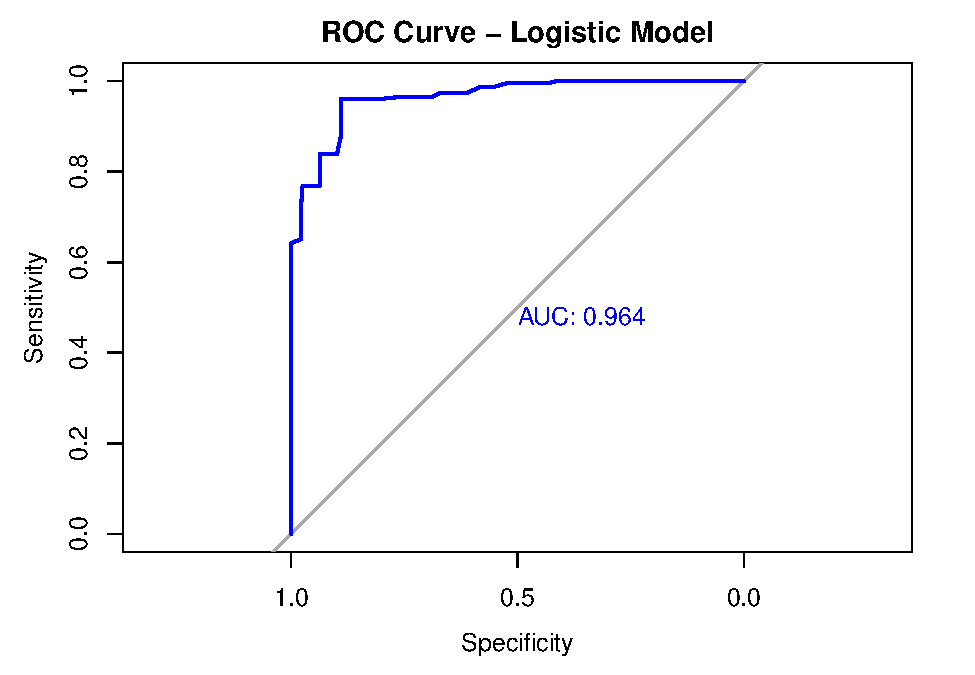
\includegraphics{HW-3-Crime-FINAL_files/figure-latex/unnamed-chunk-24-1.pdf}

\begin{Shaded}
\begin{Highlighting}[]
\NormalTok{training\_set}\SpecialCharTok{$}\NormalTok{logistic\_model }\OtherTok{\textless{}{-}} \FunctionTok{ifelse}\NormalTok{(}\FunctionTok{predict}\NormalTok{(logistic\_model, training\_set) }\SpecialCharTok{\textless{}} \FloatTok{0.5}\NormalTok{, }\DecValTok{0}\NormalTok{, }\DecValTok{1}\NormalTok{)}

\NormalTok{cm }\OtherTok{\textless{}{-}} \FunctionTok{confusionMatrix}\NormalTok{(}\FunctionTok{factor}\NormalTok{(training\_set}\SpecialCharTok{$}\NormalTok{logistic\_model), }\FunctionTok{factor}\NormalTok{(training\_set}\SpecialCharTok{$}\NormalTok{target))}
\NormalTok{results }\OtherTok{\textless{}{-}} \FunctionTok{tibble}\NormalTok{(}
  \AttributeTok{model =} \FunctionTok{character}\NormalTok{(),}
  \AttributeTok{predictors =} \FunctionTok{integer}\NormalTok{(),}
  \AttributeTok{F1 =} \FunctionTok{numeric}\NormalTok{(),}
  \AttributeTok{deviance =} \FunctionTok{numeric}\NormalTok{(),}
  \AttributeTok{r2 =} \FunctionTok{numeric}\NormalTok{(),}
  \AttributeTok{aic =} \FunctionTok{numeric}\NormalTok{()}
\NormalTok{) }

\NormalTok{results }\OtherTok{\textless{}{-}} \FunctionTok{rbind}\NormalTok{(results, }\FunctionTok{tibble}\NormalTok{(}
  \AttributeTok{model =} \StringTok{"logistic\_model"}\NormalTok{,}
  \AttributeTok{predictors =}\DecValTok{5}\NormalTok{,}
  \AttributeTok{F1 =}\NormalTok{ cm}\SpecialCharTok{$}\NormalTok{byClass[],}
  \AttributeTok{deviance =}\NormalTok{ logistic\_model}\SpecialCharTok{$}\NormalTok{deviance,}
  \AttributeTok{r2 =} \DecValTok{1} \SpecialCharTok{{-}}\NormalTok{ logistic\_model}\SpecialCharTok{$}\NormalTok{deviance }\SpecialCharTok{/}\NormalTok{ logistic\_model}\SpecialCharTok{$}\NormalTok{null.deviance,}
  \AttributeTok{aic =}\NormalTok{ logistic\_model}\SpecialCharTok{$}\NormalTok{aic}
\NormalTok{))}

\NormalTok{cm}
\end{Highlighting}
\end{Shaded}

\begin{verbatim}
## Confusion Matrix and Statistics
## 
##           Reference
## Prediction   0   1
##          0 222  53
##          1  15 176
##                                           
##                Accuracy : 0.8541          
##                  95% CI : (0.8187, 0.8849)
##     No Information Rate : 0.5086          
##     P-Value [Acc > NIR] : < 2.2e-16       
##                                           
##                   Kappa : 0.7072          
##                                           
##  Mcnemar's Test P-Value : 7.226e-06       
##                                           
##             Sensitivity : 0.9367          
##             Specificity : 0.7686          
##          Pos Pred Value : 0.8073          
##          Neg Pred Value : 0.9215          
##              Prevalence : 0.5086          
##          Detection Rate : 0.4764          
##    Detection Prevalence : 0.5901          
##       Balanced Accuracy : 0.8526          
##                                           
##        'Positive' Class : 0               
## 
\end{verbatim}

\hypertarget{model-2-1}{%
\subsubsection{model 2}\label{model-2-1}}

\begin{Shaded}
\begin{Highlighting}[]
\NormalTok{step\_model\_probs }\OtherTok{\textless{}{-}} \FunctionTok{predict}\NormalTok{(step\_model, }\AttributeTok{type =} \StringTok{"response"}\NormalTok{)}
\NormalTok{roc\_curve\_step }\OtherTok{\textless{}{-}} \FunctionTok{roc}\NormalTok{(training\_set}\SpecialCharTok{$}\NormalTok{target, step\_model\_probs)}
\end{Highlighting}
\end{Shaded}

\begin{verbatim}
## Setting levels: control = 0, case = 1
\end{verbatim}

\begin{verbatim}
## Setting direction: controls < cases
\end{verbatim}

\begin{Shaded}
\begin{Highlighting}[]
\FunctionTok{plot}\NormalTok{(roc\_curve\_step, }\AttributeTok{main =} \StringTok{"ROC Curve {-} Step Model"}\NormalTok{, }\AttributeTok{col =} \StringTok{"red"}\NormalTok{, }\AttributeTok{print.auc =} \ConstantTok{TRUE}\NormalTok{)}
\end{Highlighting}
\end{Shaded}

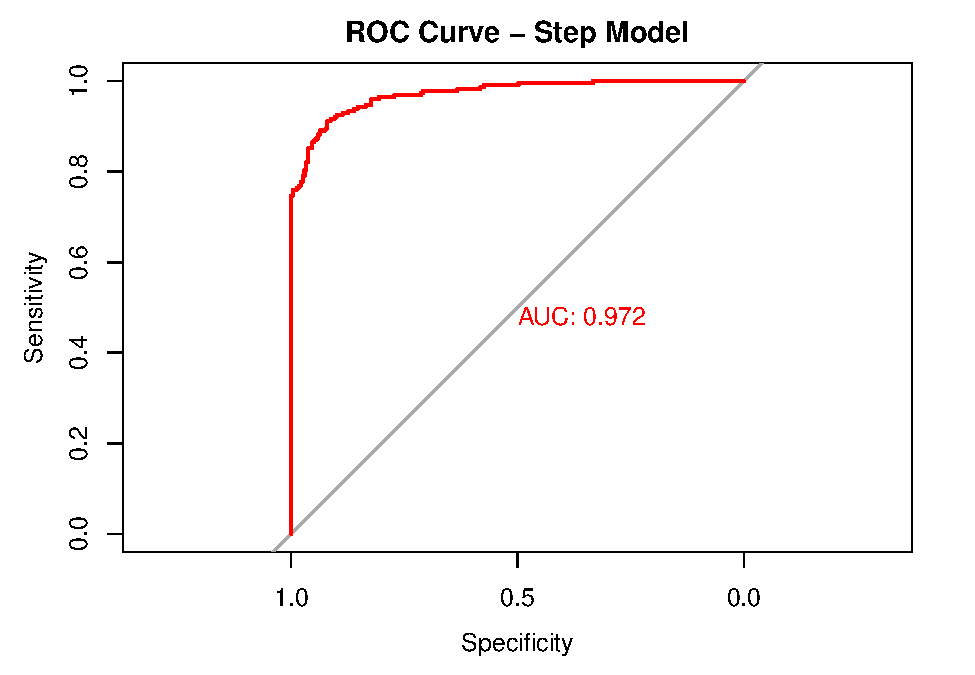
\includegraphics{HW-3-Crime-FINAL_files/figure-latex/unnamed-chunk-26-1.pdf}

\begin{Shaded}
\begin{Highlighting}[]
\NormalTok{training\_set}\SpecialCharTok{$}\NormalTok{step\_model }\OtherTok{\textless{}{-}} \FunctionTok{ifelse}\NormalTok{(}\FunctionTok{predict}\NormalTok{(step\_model, training\_set) }\SpecialCharTok{\textless{}} \FloatTok{0.5}\NormalTok{, }\DecValTok{0}\NormalTok{, }\DecValTok{1}\NormalTok{)}
\NormalTok{cm\_step\_model }\OtherTok{\textless{}{-}} \FunctionTok{confusionMatrix}\NormalTok{(}\FunctionTok{factor}\NormalTok{(training\_set}\SpecialCharTok{$}\NormalTok{step\_model), }\FunctionTok{factor}\NormalTok{(training\_set}\SpecialCharTok{$}\NormalTok{target))}

\NormalTok{results }\OtherTok{\textless{}{-}} \FunctionTok{rbind}\NormalTok{(results, }\FunctionTok{tibble}\NormalTok{(}
  \AttributeTok{model =} \StringTok{"step\_model"}\NormalTok{,}
  \AttributeTok{predictors =} \DecValTok{8}\NormalTok{, }
  \AttributeTok{F1 =}\NormalTok{ cm\_step\_model}\SpecialCharTok{$}\NormalTok{byClass[}\StringTok{"F1"}\NormalTok{],}
  \AttributeTok{deviance =}\NormalTok{ step\_model}\SpecialCharTok{$}\NormalTok{deviance,}
  \AttributeTok{r2 =} \DecValTok{1} \SpecialCharTok{{-}}\NormalTok{ step\_model}\SpecialCharTok{$}\NormalTok{deviance }\SpecialCharTok{/}\NormalTok{ step\_model}\SpecialCharTok{$}\NormalTok{null.deviance,}
  \AttributeTok{aic =}\NormalTok{ step\_model}\SpecialCharTok{$}\NormalTok{aic}
\NormalTok{))}

\NormalTok{cm\_step\_model}
\end{Highlighting}
\end{Shaded}

\begin{verbatim}
## Confusion Matrix and Statistics
## 
##           Reference
## Prediction   0   1
##          0 237 227
##          1   0   2
##                                           
##                Accuracy : 0.5129          
##                  95% CI : (0.4665, 0.5591)
##     No Information Rate : 0.5086          
##     P-Value [Acc > NIR] : 0.4448          
##                                           
##                   Kappa : 0.0089          
##                                           
##  Mcnemar's Test P-Value : <2e-16          
##                                           
##             Sensitivity : 1.000000        
##             Specificity : 0.008734        
##          Pos Pred Value : 0.510776        
##          Neg Pred Value : 1.000000        
##              Prevalence : 0.508584        
##          Detection Rate : 0.508584        
##    Detection Prevalence : 0.995708        
##       Balanced Accuracy : 0.504367        
##                                           
##        'Positive' Class : 0               
## 
\end{verbatim}

\hypertarget{model-3-1}{%
\subsubsection{Model 3}\label{model-3-1}}

\begin{Shaded}
\begin{Highlighting}[]
\NormalTok{step\_model3\_probs }\OtherTok{\textless{}{-}} \FunctionTok{predict}\NormalTok{(step\_model3, }\AttributeTok{type =} \StringTok{"response"}\NormalTok{)}
\NormalTok{roc\_curve\_step\_model3 }\OtherTok{\textless{}{-}} \FunctionTok{roc}\NormalTok{(training\_set}\SpecialCharTok{$}\NormalTok{target, step\_model3\_probs)}
\end{Highlighting}
\end{Shaded}

\begin{verbatim}
## Setting levels: control = 0, case = 1
\end{verbatim}

\begin{verbatim}
## Setting direction: controls < cases
\end{verbatim}

\begin{Shaded}
\begin{Highlighting}[]
\FunctionTok{plot}\NormalTok{(roc\_curve\_step\_model3, }\AttributeTok{col =} \StringTok{"green"}\NormalTok{, }\AttributeTok{print.auc =} \ConstantTok{TRUE}\NormalTok{)}
\end{Highlighting}
\end{Shaded}

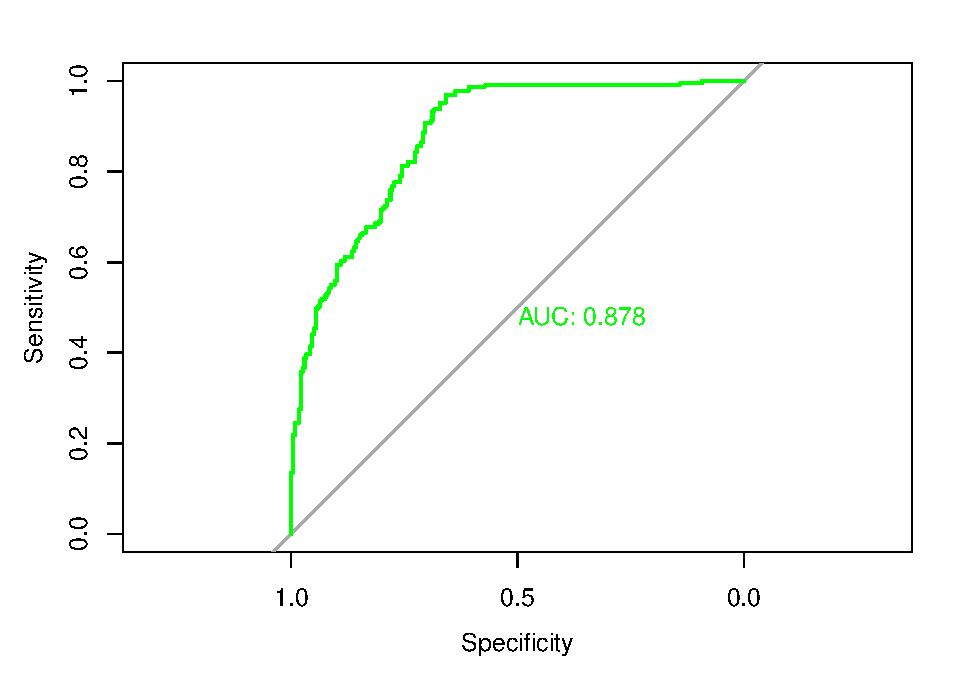
\includegraphics{HW-3-Crime-FINAL_files/figure-latex/unnamed-chunk-28-1.pdf}

\begin{Shaded}
\begin{Highlighting}[]
\NormalTok{training\_set}\SpecialCharTok{$}\NormalTok{step\_model3 }\OtherTok{\textless{}{-}} \FunctionTok{ifelse}\NormalTok{(}\FunctionTok{predict}\NormalTok{(step\_model3, training\_set) }\SpecialCharTok{\textless{}} \FloatTok{0.5}\NormalTok{, }\DecValTok{0}\NormalTok{, }\DecValTok{1}\NormalTok{)}

\NormalTok{cm\_step\_model3 }\OtherTok{\textless{}{-}} \FunctionTok{confusionMatrix}\NormalTok{(}\FunctionTok{factor}\NormalTok{(training\_set}\SpecialCharTok{$}\NormalTok{step\_model3), }\FunctionTok{factor}\NormalTok{(training\_set}\SpecialCharTok{$}\NormalTok{target))}

\NormalTok{results }\OtherTok{\textless{}{-}} \FunctionTok{rbind}\NormalTok{(results, }\FunctionTok{tibble}\NormalTok{(}
  \AttributeTok{model =} \StringTok{"step\_model3"}\NormalTok{,}
  \AttributeTok{predictors =} \DecValTok{4}\NormalTok{, }
  \AttributeTok{F1 =}\NormalTok{ cm\_step\_model3}\SpecialCharTok{$}\NormalTok{byClass[}\StringTok{"F1"}\NormalTok{],}
  \AttributeTok{deviance =}\NormalTok{ step\_model3}\SpecialCharTok{$}\NormalTok{deviance,}
  \AttributeTok{r2 =} \DecValTok{1} \SpecialCharTok{{-}}\NormalTok{ step\_model3}\SpecialCharTok{$}\NormalTok{deviance }\SpecialCharTok{/}\NormalTok{ step\_model3}\SpecialCharTok{$}\NormalTok{null.deviance,}
  \AttributeTok{aic =}\NormalTok{ step\_model3}\SpecialCharTok{$}\NormalTok{aic}
\NormalTok{))}

\NormalTok{cm\_step\_model3}
\end{Highlighting}
\end{Shaded}

\begin{verbatim}
## Confusion Matrix and Statistics
## 
##           Reference
## Prediction   0   1
##          0 189  64
##          1  48 165
##                                           
##                Accuracy : 0.7597          
##                  95% CI : (0.7182, 0.7978)
##     No Information Rate : 0.5086          
##     P-Value [Acc > NIR] : <2e-16          
##                                           
##                   Kappa : 0.5186          
##                                           
##  Mcnemar's Test P-Value : 0.1564          
##                                           
##             Sensitivity : 0.7975          
##             Specificity : 0.7205          
##          Pos Pred Value : 0.7470          
##          Neg Pred Value : 0.7746          
##              Prevalence : 0.5086          
##          Detection Rate : 0.4056          
##    Detection Prevalence : 0.5429          
##       Balanced Accuracy : 0.7590          
##                                           
##        'Positive' Class : 0               
## 
\end{verbatim}

Based on the provided metrics, Model 1 (logistic\_model) demonstrates
the highest accuracy of 85.41\% compared to Model 2 (step\_model) and
Model 3 (step\_model3), which have accuracies of 51.29\% and 75.97\%,
respectively. Additionally, Model 1 exhibits strong precision (80.73\%)
and sensitivity (93.67\%), indicating its ability to correctly identify
true positives and minimize false positives. Moreover, Model 1 achieves
a balanced accuracy of 85.26\%, reflecting its robust performance across
both positive and negative classes. In contrast, Model 2 shows limited
performance with a precision of 51.08\% and sensitivity of 100\%,
suggesting potential overfitting or inadequate generalization. Model 3,
although better than Model 2, lags behind Model 1 in accuracy and
sensitivity, indicating room for improvement. Therefore, based on the
provided metrics, Model 1 (logistic\_model) appears to be the superior
choice due to its higher accuracy, precision, sensitivity, and balanced
performance across classes.

\end{document}
